\documentclass[a4paper, 12pt]{article} % 12pt, A4 page

% packages
\usepackage{amsmath} % math symbols
\usepackage{amsfonts} % 〃    〃
\usepackage{amsthm} % math proofs
\usepackage{xcolor} % text coloring
\usepackage{setspace} % spacing
\usepackage{graphicx} % image
\usepackage{cite} % BibTex
\usepackage[notlof,nottoc,numbib]{tocbibind} % somehow makes the references appear in ToC

\newcommand{\researchquestion}{How can vector calculus be used to model and analyze incompressible fluid flow in two-dimensional spaces, and what insights can this provide about the vector fields of real-world fluid systems with circular obstacles?}
\graphicspath{ {resources/} }

% custom commands
\newcommand{\ihat}{\hat{\imath}} % i hat
\newcommand{\jhat}{\hat{\jmath}} % j hat
\newcommand{\fatf}{\mathbf{F}} % for Vector field F
\newcommand{\definedas}{\stackrel{\Delta}{=}} % definitions
\newcommand{\referto}[1]{\textsuperscript{\color{darkgray}\tiny[see \ref{#1}]}} % definitions
% > derivatives
\newcommand{\der}[2]{\frac{\mathrm{d} #1}{\mathrm{d} #2}} % derivative
\newcommand{\partialder}[2]{\frac{\partial #1}{\partial #2}} % partial derivative
\newcommand{\materialder}[2]{\frac{\mathrm{D} #1}{\mathrm{D} #2}} % material derivative
% > vector calculus operators
\DeclareMathOperator{\gradient}{\nabla} % gradient operator
\DeclareMathOperator{\divergence}{\nabla\cdot} % divergence operator
\DeclareMathOperator{\curl}{\nabla\times} % divergence operator

% formatting
\doublespacing % double spacing
\pagenumbering{arabic} % page numbering

% theorems
\newtheorem{greenstheorem}{Green's theorem}

\begin{document}
\begin{titlepage} % title page
	\begin{center}
		\vspace*{0.5cm}
		\Large
		\textbf{\researchquestion}

		\vspace{1.5cm}
		\large
		\textbf{Mathematics AA HL}

		\vfill{}\color{darkgray}
		Word Count: 396 % (maximum 4000)
	\end{center}
\end{titlepage}

\tableofcontents\newpage % table of contents

% INTRODUCTION
\section{Introduction}
Vector calculus provides the foundation and tools for the analysis and modeling of several real-world phenomona, and is integral to understanding several important fields such as aero- \& hydrodynamics, as well as the modeling of weather \& climates. 

Through the use of pure mathematics, this essay will investigate the flow of fluids in 2 dimensional spaces around circular obstacles. Visual representations through mediums such as vector field plots (plotted through a custom program
% > aim & scope
\subsection{Aim \& scope}
This essay will for simplicity's sake only cover fluid flow around circular obstacles in $\mathbb{R}^2$ spaces; an alaysis of fluid flow in $\mathbb{R}^3$ spaces would be much more complex.
Furthermore, only incompressible fluids sans sinks and sources ($\fatf\ni\divergence\fatf=0$), will be analyzed.

Most of the analysis will take place using Green's theorem\referto{sec:greenstheorem}.

% > background
\subsection{Background}
Vector calculus is the mathematical study of applying multi-variable calculus to vector valued functions, often for the spaces $\mathbb{R}^2$ and $\mathbb{R}^3$.

\subsubsection{The gradient operator}
In one dimensional calculus, the gradient (slope) of a graph can be calculated at any point by differentiating the function and evaluating it at said point. 
$$f(x)=x^2\implies\der{f}{x}=2x$$
Defining this as the equation of greatest incline at point $x$, even though there in this case is only one true rate of the function since we are working in the space $\mathbb{R}^1$, will help us when extending this concept of greatest incline to $\mathbb{R}^n$ spaces.

In multi-variable calculus a new tool called the partial derivative helps us differentiate multi-variable functions. It works identically to a regular derivative just that we treat all variables other than the one we are differentiating with respect to as constants.
$$f(x,y)=x^2+y^2\implies\partialder{f}{x}=2x$$
This finds the greatest change the equation of greatest change for $f$ in the direction differentiated by, so if we combine the partial derivatives in all directions $f$ takes as parameters into a vector, then we end up with the equation of steepest descent.

The gradient operator, denoted by the symbol $\nabla$ (pronounced nabla or grad), is thereby defined for some function $f:\mathbb{R}^n\rightarrow\mathbb{R}^m$ as:
\begin{equation}
	\left.\nabla=
	\begin{bmatrix}
		\partialder{}{x} \\
		\partialder{}{y} \\
		\partialder{}{z} \\ 
		\vdots 	         \\
	\end{bmatrix}
	\color{gray}\right\} \color{gray}n\text{ times}\color{black}
\end{equation}
Aplying this to our previous example $f(x,y)=x^2+y^2$, then we get:
$$\nabla f=\begin{bmatrix}
	\partialder{}{x}x^2+y^2\\
	\partialder{}{y}x^2+y^2	
\end{bmatrix}=\begin{bmatrix}
	2x\\
	2y
\end{bmatrix}$$
Meaning that at some point $(x,y)$, the direction of steepest incline will be $2(x,y)$. The nabla operator proves foundational to vector calculus and is the backbone of several important concepts.

\subsubsection{Other}
$$f:\mathbb{R}^n\rightarrow\mathbb{R}^n\ni n>1,n\in\mathbb{Z}$$
\begin{equation}
	\materialder{f}{t}\definedas\partialder{f}{t}+\vec{v}\cdot\nabla f
\end{equation}
$$\vec{v_1}\otimes\vec{v_2}$$

% > fluid dynamics
\subsection{Fluid dynamics}
An incompressible fluid is any fluid such that $\divergence\fatf=0$, which is to say that the divergence of the fluid is 0.

% > the navier-stokes equations
\subsection{Green's theorem}\label{sec:greenstheorem}
\begin{greenstheorem}
	The double integral over some reigon $R$ of the curl of a vector field $\fatf$ is equal to the line integral over some curve $C$ of $\fatf$
	$$\int_C \mathbf{F} \cdot d\mathbf{r} = \iint_R \left( \frac{\partial Q}{\partial x} - \frac{\partial P}{\partial y} \right) \, dA$$
	$$\iint_R\curl\fatf\mathrm{d}A=\oint_C\fatf\cdot\mathrm{d}\mathbf{r}$$
\end{greenstheorem}
\begin{equation} % navier-stokes
	\materialder{f}{\mathbf{t}}=\iiint\limits_{V}(\materialder{\rho}{\mathbf{t}}+\rho(\nabla\cdot u))dV
\end{equation}
Lorem ipsum dolor sit amet \cite{peyret2012computational}

% references
\newpage
\bibliographystyle{apalike}
\bibliography{sources}
\stepcounter{section}
\addcontentsline{toc}{section}{\protect\numberline{\thesection}List of Figures}
\renewcommand{\listfigurename}{\thesection\hspace{20pt}List of Figures}\listoffigures

% testing
\newpage
\begin{figure}
	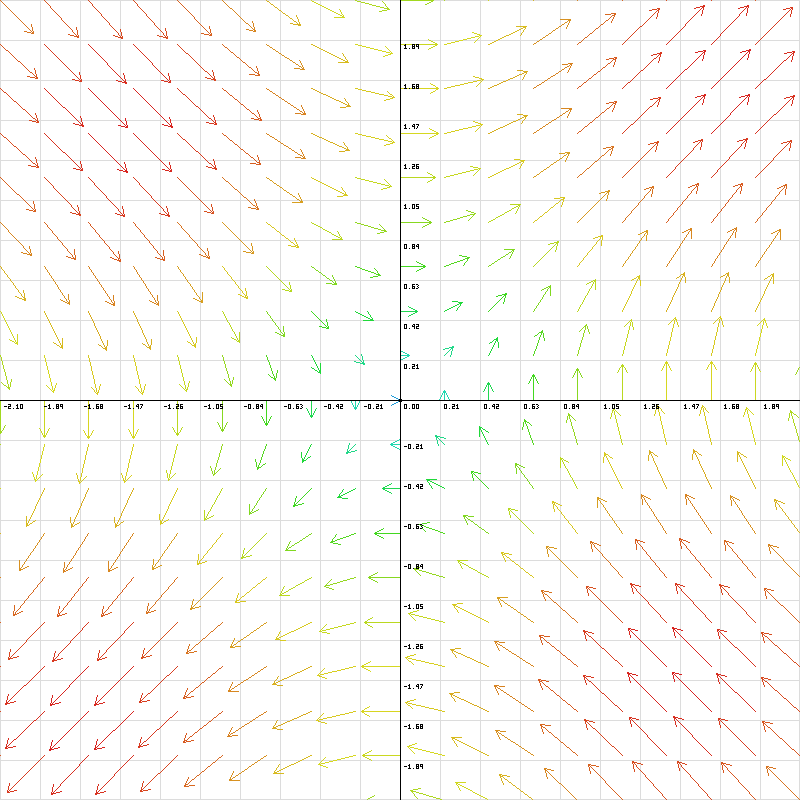
\includegraphics[scale=0.45]{sin.png}
	\centering
	\caption{Vector field for $f(x,y)=\begin{pmatrix}\sin y\\\sin x\end{pmatrix}$}
	\label{fig:Banana}
\end{figure}
$$\fatf(t):\mathbb{R}\rightarrow\mathbb{R}^2$$
$$\leadsto\mathbf{P}(t, \vec{p})=\vec{p}+\hat{\imath}\iint_0^t\fatf_x\ \mathrm{d}t+\hat{\jmath}\iint_0^t\fatf_y\ \mathrm{d}t$$
$$\mathbf{P}(t, \vec{p})=\vec{p}+\iint_0^t\hat{\imath}\fatf_x+\hat{\jmath}\fatf_y\ \mathrm{d}t$$
$$\jhat+\ihat$$
\begin{align*}
	A&=B\\
	 &=C && \text{substitution}
\end{align*}
\begin{proof} Green's Theorem
	\begin{align*}
		B \definedas C \span \\
		A&=B \\
		 &=C \\
	\end{align*}
\end{proof}
$$a\underbrace{a}_\text{banana}$$
\end{document}